\documentclass[extra,mreferee]{gji}
%\documentclass[extra]{gji}
\usepackage{timet}
\usepackage{amsmath}
\usepackage{graphicx}
\usepackage{url}
\usepackage[utf8]{inputenc}
% To make two column figures appear in the correct order
\usepackage{fixltx2e}
% To make annotations on the sides
\usepackage{todonotes}

% Document metadata
%%%%%%%%%%%%%%%%%%%%%%%%%%%%%%%%%%%%%%%%%%%%%%%%%%%%%%%%%%%%%%%%%%%%%%%%%%%%%%%
\newcommand{\Title}{
    Fast non-linear gravity inversion in spherical coordinates
    with application to the South American Moho
}
\newcommand{\Keywords}{
    Inverse theory;
    Gravity anomalies and Earth structure;
    Satellite gravity;
    South America;
}
\title[]{\Title}
\author[]{
    Leonardo Uieda$^{1,2}$,
    Valéria C. F. Barbosa$^{2}$
    \\
    $^1$Universidade do Estado do Rio de Janeiro, Rio de Janeiro, Brazil.
    e-mail: leouieda@gmail.com
    \\
    $^2$Observatório Nacional, Rio de Janeiro, Brazil.
}
% Metadata for the generated PDF
\usepackage[pdftex,colorlinks=true]{hyperref}
\hypersetup{
    pdftitle={\Title},
    pdfauthor={Leonardo Uieda (leouieda@gmail.com)},
    pdfsubject={},
    pdfkeywords={\Keywords},
    pdfcreator={pdfTeX},
    allcolors=blue,
}


\begin{document}


\label{firstpage}
\maketitle


\begin{abstract}
    Estimating the relief of the Moho from gravity data is a computationally
    intensive non-linear inverse problem.
    What is more, the modeling must take the Earths curvature into account when
    the study area is of regional scale or greater.
    We present a regularized non-linear gravity inversion method that has a low
    computational footprint and employs a spherical Earth approximation.
    To achieve this, we combine the highly efficient Bott's method with
    smoothness regularization and a discretization of the anomalous Moho into
    tesseroids (spherical prisms).
    The computational efficiency of our method is attained by harnessing the
    fact that all matrices involved are sparse.
    The inversion results are controlled by three hyper-parameters: the
    regularization parameter, the anomalous Moho density-contrast, and the
    reference Moho depth.
    We estimate the regularization parameter using the method of hold-out
    cross-validation.
    Additionally, we estimate the density-contrast and the reference depth
    using knowledge of the Moho depth at certain points.
    We apply the proposed method to estimate the Moho depth for the South
    American continent using satellite gravity data and seismological data.
    The final Moho model is in accordance with previous gravity-derived models
    and seismological data.
    The misfit to the gravity and seismological data is worse in the Andes and
    best in oceanic areas, central Brazil and Patagonia, and along the Atlantic
    coast.
    Similarly to previous results, the model suggests a thinner crust of 30-35
    km under the Andean foreland basins.
    Discrepancies with the seismological data are greatest in the Guiana
    shield, the central Solimões and Amazon Basins, the Paraná Basin, and the
    Borborema province.
    These differences suggest the existence of crustal or mantle density
    anomalies that were unaccounted for during gravity data processing.
\end{abstract}


\noindent\textbf{Key words:} \Keywords


%%%%%%%%%%%%%%%%%%%%%%%%%%%%%%%%%%%%%%%%%%%%%%%%%%%%%%%%%%%%%%%%%%%%%%%%%%%%%%%
\section{Introduction}

The Mohorovičić discontinuity (or Moho) that marks the transition from the
crust to the mantle, is studied almost exclusively through indirect geophysical
methods.
The two main geophysical methods used to estimate the depth of the Moho are
seismology, with both natural and controlled sources, and gravimetry.
With the advent of satellite gravimetry missions like GRACE and GOCE,
gravity-derived crustal models can be produced in regional or global scales
\citep[e.g. ][]{reguzzoni2013,vandermeijde2013,vandermeijde2015}.
New spherical harmonic gravity models that use these satellite observation,
like GOCO5S \citep{mayer-guerr2015}, provide almost homogeneous data coverage
in difficult to access regions traditionally poor in terrestrial data.
An example is South America, where seismologic and terrestrial gravity data
are traditionally concentrated around urban centers and coastal areas,
resulting in large areas (e.g., forests and mountains) devoid of data.

Estimating Moho depth from gravity data is a non-linear inverse problem.
One can generalize this problem of estimating the depths of an interface
separating two media,
such as the sediment-basement interface of a sedimentary basin or the
crust-mantle interface (Moho).
Several methods have been developed over the years to solve this inverse
problem, for example
\citet{bott1960, barbosa1999b, barbosa1999a, barnes2012, leao1996, martins2010,
martins2011, oldenburg1974, reguzzoni2013, santos2015, silva2006, silva2014},
to name a few.
Solving the inverse problem is computationally demanding because it requires
the construction of large dense matrices and the solution of large linear
systems.
As a result, some authors search for ways to increase the computational
efficiency of this class of inverse problem.
\citet{bott1960} proposed a method based on iteratively applying corrections to
a starting estimate based on the inversion residuals.
The algorithm is fast because it bypasses the construction and solution of
linear systems and only involves forward modeling.
\citet{oldenburg1974} showed that the fast FFT-based forward modeling of
\citet{parker1973} could be rearranged to estimate the relief.
\citet{barnes2012} use a form of adaptive discretization to compute the
Jacobian, or sensitivity, matrix.
For each data point, the discretization will be progressively coarser
the further way from the point.
This reduces the matrix and, consequently, the linear systems to a sparse form
that can be solved efficiently.
Recently, \citet{silva2014} extended and generalized the original method of
\citet{bott1960} and \citet{santos2015} used this extension to estimate a
basement relief with sharp boundaries.

A spherical Earth approximation is preferred when estimating the Moho depth
from gravity data in continental and global scale studies.
\citet{wieczorek1998} developed a spherical harmonic equivalent of the
Parker-Oldenburg FFT algorithm and applied it to estimate the crustal structure
of the Moon.
\citet{reguzzoni2013} use a spherical Earth approximation to estimate the
global Moho relief using data from the GOCE satellite mission.
Another approach is to use
non-spectral (space domain) gravity inversion methods.
Many such methods were developed for estimating the basement relief of a
sedimentary basin
\citep[e.g., ][]{barbosa1999a, barbosa1999b, martins2010, martins2011, sun2014}.
These methods approximate the sedimentary pack by a set of juxtaposed
right-rectangular prisms.
The top of the prisms coincide with the Earth's surface and the prisms'
thicknesses represent the depths to the basement and are the parameters to be
estimated in the inversion.
The use of rectangular prisms implies a planar Earth approximation and may not
be adequate for depth-to-Moho estimates in a continental-scale study.
A straightforward way to circumvent this hindrance is to adapt one of the
methods developed for rectangular prisms to use tesseroids (spherical prisms).
One of the difficulties of this approach is that the forward problem for a
tesseroid must be solved numerically.
Two alternatives proposed in the literature to the numerical solution are
Taylor series expansion \citep{heck2007, grombein2013}
and the Gauss-Legendre Quadrature
\citep{asgharzadeh2007}.
Numerical experiments by \citet{wild-pfeiffer2008} suggest that the
Gauss-Legendre Quadrature (GLQ) offers superior results.
However, the GLQ suffers from numerical instability when the computation point
is close to the tesseroid \citep{asgharzadeh2007}.
To overcome the numerical instability, \citet{li2011} proposed an adaptive
discretization algorithm which was later improved upon by \citet{uieda2016}.

In any gravity inversion for estimating the relief of an interface, two
hyper-parameters control the inversion results: the density-contrast between
the two media and the reference level around which the interface undulates.
The reference level is the constant depth of the Normal Earth Moho in the case
of the anomalous Moho.
For regularized inversions, an additional hyper-parameter is the regularization
parameter that balances the relative importance between the data-misfit measure
and the regularizing function.
The two most commonly used methods for estimating the regularization parameter
are the L-curve criterion and Generalized Cross Validation (GCV).
\citet{farquharson2004} provide for a thorough comparison of both methods.
Estimating the density-contrast in a sedimentary basin context has been tackled
by \citet{silva2006} and \citet{martins2010} when the basement depth is known
at a few points.
To the authors' knowledge no attempt has been made to estimate the reference
level.

We present a non-linear gravity inversion to estimate the Moho depth in
a spherical Earth approximation.
Our method is based on the \citet{silva2014} Gauss-Newton formulation of the
method of \citet{bott1960}.
We use tesseroids to discretize the anomalous Moho and the adaptive
discretization algorithm of \citet{uieda2016} for the forward modeling.
The stability of the inversion is achieved through smoothness regularization.
In order to maintain the computational efficiency of Bott's method,
we exploit the sparse nature of all matrices involved in the computations.
We employ a variant of GCV known as hold-out cross-validation \citep{kim2009}
to estimate the regularization parameter.
Additionally, we estimate the density-contrast and reference level
simultaneously in a second cross-validation.
Similarly to \citet{silva2006} and \citet{martins2010}, this cross-validation
procedure uses knowledge of the Moho depths at certain points.
Finally, we apply the proposed method to estimate the Moho depth for South
America using gravity data from the GOCO5S model \citep{mayer-guerr2015} and
the seismological data of \citet{assumpcao2013a}.



%%%%%%%%%%%%%%%%%%%%%%%%%%%%%%%%%%%%%%%%%%%%%%%%%%%%%%%%%%%%%%%%%%%%%%%%%%%%%%%
\section{Methodology}

In potential field methods, we must isolate the target anomalous density
distribution before modeling and inversion.
In our case, the target is the relief of the real Moho undulating around a
reference Moho.
We do this by removing all other effects from the gravity observations.
The first correction is to remove the
scalar gravity of an ellipsoidal reference Earth (the Normal Earth),
hereafter denoted as $\gamma$.
This effect is calculated on the same point $P$ where
the gravity observation was made
(Fig~\ref{fig:anomalysketch}a-b).
$\gamma(P)$ is calculated using
the closed-form solution presented by \citet{li2001a}.
The difference between the observed gravity at point P ($g(P)$)
and Normal gravity at the same point
is known as the gravity disturbance,

\begin{equation}
    \delta(P) = g(P) - \gamma(P).
    \label{eq:disturbance}
\end{equation}

The disturbance contains only the gravitational effects of density
distributions that are anomalous with respect to the Normal Earth
(see Fig.~\ref{fig:anomalysketch}c).
This includes all masses above the surface of the ellipsoid (the topography),
the mass deficiency of the oceans,
the mass deficiency of sedimentary basins,
crustal sources (e.g., igneous intrusions, lateral density changes, etc),
heterogeneities below the upper mantle,
and the effect of the difference between the real Moho
topography and the Moho of the Normal Earth.

To estimate the anomalous Moho relief from gravity data,
we must first isolate its gravitational attraction.
Thus, all other gravitational effects
must be either removed or assumed negligible.
Here, we will remove the gravitational effect produced by the known topography
and ocean masses to obtain the full Bouguer disturbance
(Fig~\ref{fig:anomalysketch}d),

\begin{equation}
    \delta_{bg}(P) = \delta(P) - g_{topo}(P).
    \label{eq:bouguer}
\end{equation}

\noindent
We will also remove the gravitational effect of know sedimentary basins
but assume that the effects of
other crustal and mantle sources are negligible.
Thus, the only effect left will be that of the anomalous Moho relief
(Fig~\ref{fig:anomalysketch}e).
The gravitational attraction of the topography, oceans, and basins are
calculated in a spherical Earth approximation by forward modeling using
tesseroids (Fig.~\ref{fig:tesseroid}).
The tesseroid effects are calculated numerically using
Gauss-Legendre Quadrature (GLQ) integration \citep{asgharzadeh2007}.
The accuracy of the GLQ integration is improved by the adaptive discretization
scheme of \citet{uieda2016}.


\begin{figure}
    \centering
    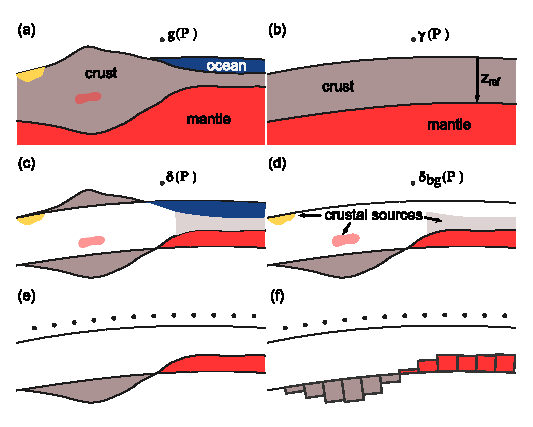
\includegraphics{figures/problem-concept}
    \caption{
        Sketch of the stages in gravity data correction and
        the discretization of the anomalous Moho relief using tesseroids.
        (a) The Earth and the measured gravity at point P ($g(P)$).
        (b) The Normal Earth and the calculated normal gravity at point P
        ($\gamma(P)$). $z_{ref}$ is the depth of the Normal Earth Moho.
        (c) The gravity disturbance ($\delta(P)$) and the corresponding density
        anomalies after removal of the normal gravity: topography, oceans,
        crustal and mantle heterogeneities, and the anomalous Moho.
        (d) The Bouguer disturbance ($\delta_{bg}(P)$) after topographic
        correction and the remaining density anomalies.
        (e) All density anomalies save the anomalous Moho are assumed to have
        been removed before inversion.
        (f) The discretization of the anomalous Moho in tesseroids. Grey
        tesseroids will have a negative density contrast while red tesseroids
        will have a positive one.
    }
    \label{fig:anomalysketch}
\end{figure}

\begin{figure}
    \centering
    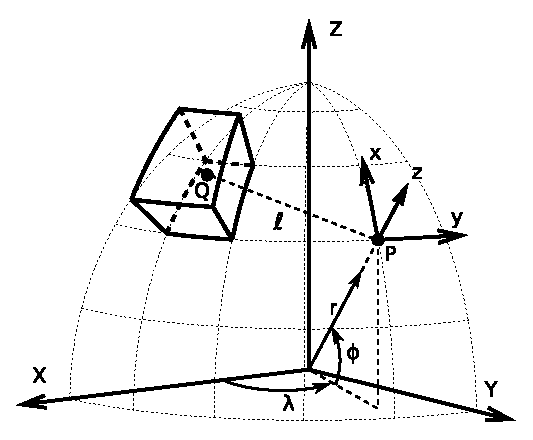
\includegraphics{figures/tesseroid-coord-sys}
    \caption{Sketch of a tesseroid (spherical prism) in a geocentric coordinate
        system (X, Y, Z).
        Observations are made at point P with respect to it's local
        North-oriented coordinate system (x, y, z).
        After \citet{uieda2015}.
    }
    \label{fig:tesseroid}
\end{figure}


%%%%%%%%%%%%%%%%%%%%%%%%%%%%%%%%%%%%%%%%%%%%%%%%%%%%%%%%%%%%%%%%%%%%%%%%%%%%%%%
\subsection{Parametrization and the forward problem}

We parameterize the forward problem by discretizing the anomalous Moho
into a grid of $M_{lon} \times M_{lat} = M$ juxtaposed tesseroids
(Fig~\ref{fig:anomalysketch}f).
The true (real Earth) Moho varies in depth
with respect to the Moho of the Normal Earth.
Hereafter we will refer to the depth of the Normal Earth Moho as $z_{ref}$
(see Fig.~\ref{fig:anomalysketch}b).
If the true Moho is above $z_{ref}$,
the top of the $k$th tesseroid is the Moho depth $z_{k}$,
the bottom is $z_{ref}$, and the density-contrast ($\Delta\rho$) is positive
(red tesseroids in Fig~\ref{fig:anomalysketch}f).
If the Moho is below $z_{ref}$, the top of the tesseroid is $z_{ref}$,
the bottom is $z_k$, and $\Delta\rho$ is negative
(grey tesseroids in Fig~\ref{fig:anomalysketch}f).

Considering that the absolute value of the density-contrasts
of the tesseroids is a fixed parameter,
the predicted gravity anomaly of the Moho is a non-linear function of the
parameters $z_k$, $k=1, \ldots, M$,

\begin{equation}
    d_i = f_i(\mathbf{p}),
    \label{eq:forward}
\end{equation}

\noindent in which $d_i$ is the $i$th element of the $N$-dimensional predicted
data vector $\mathbf{d}$, $\mathbf{p}$ is the $M$-dimensional parameter vector
containing the $M$ Moho depths ($z_k$),
and $f_i$ is the $i$th non-linear function that maps the parameters onto the
data.
The functions $f_i$ are the radial component of the gravitational attraction
of the tesseroid Moho model.



%%%%%%%%%%%%%%%%%%%%%%%%%%%%%%%%%%%%%%%%%%%%%%%%%%%%%%%%%%%%%%%%%%%%%%%%%%%%%%%
\subsection{Inverse problem}

We wish to estimate the parameter vector $\mathbf{p}$ from a set of observed
gravity data $\mathbf{d}^o$.
The least-squares estimate is the one that minimizes the data-misfit function

\begin{equation}
    \phi(\mathbf{p}) =
        [\mathbf{d}^o - \mathbf{d}(\mathbf{p})]^T
        [\mathbf{d}^o - \mathbf{d}(\mathbf{p})].
    \label{eq:data-misfit}
\end{equation}

Function $\phi(\mathbf{p})$ is non-linear with respect to $\mathbf{p}$.
Thus, we can determine its minimum using gradient-based
iterative optimization
methods like Gauss-Newton or Steepest Descent.
Such methods start from an initial approximation to the model parameter vector
$\mathbf{p}^0$ and estimate a parameter perturbation vector
$\mathbf{\Delta p}^0$.
The perturbation vector is used to update $\mathbf{p}^0$ to
$\mathbf{p}^1 =  \mathbf{p}^0 + \mathbf{\Delta p}^0$.
This procedure is repeated until a minimum of function $\phi(\mathbf{p})$
(Eq.~\ref{eq:data-misfit}) is reached.

For the Gauss-Newton method,
the parameter perturbation vector at the $k$th iteration $\mathbf{\Delta p}^k$
is obtained by solving the linear system

\begin{equation}
    \mathbf{H}^k\mathbf{\Delta p}^k = -\mathbf{\nabla\phi}^k,
    \label{eq:gaussnewton}
\end{equation}

\noindent in which
$\mathbf{\nabla\phi}^k$ and $\mathbf{H}^k$ are, respectively,
the gradient vector and the Hessian matrix of $\phi(\mathbf{p})$.

The gradient vector and the Gauss-Newton approximation of the Hessian matrix
of $\phi(\mathbf{p})$ are, respectively,

\begin{equation}
    \mathbf{\nabla\phi}^k = -2{\mathbf{A}^k}^T[\mathbf{d}^o - \mathbf{d}(\mathbf{p}^k)],
    \label{eq:gradient}
\end{equation}

\noindent
and

\begin{equation}
    \mathbf{H}^k \approx 2{\mathbf{A}^k}^T{\mathbf{A}^k},
    \label{eq:hessian}
\end{equation}

\noindent in which
$\mathbf{A}^k$ is the $N \times M$ Jacobian or sensitivity matrix
whose elements are

\begin{equation}
    A_{ij}^k = \dfrac{\partial f_i}{\partial p_j}(\mathbf{p}^k).
    \label{eq:jacobian}
\end{equation}



%%%%%%%%%%%%%%%%%%%%%%%%%%%%%%%%%%%%%%%%%%%%%%%%%%%%%%%%%%%%%%%%%%%%%%%%%%%%%%%
\subsection{Regularization}

Non-linear gravity inversions for estimating the relief of an interface
separating two media (like the Moho) are ill-posed and require additional
constraints in the form of regularization \citep{silva2001b}.
A common approach is to use the first-order Tikhonov regularization
\citep{tikhonov1977} to impose smoothness on the solution.
The cost function for smoothness regularization is given by

\begin{equation}
    \theta(\mathbf{p}) = \mathbf{p}^T\mathbf{R}^T\mathbf{R}\mathbf{p},
    \label{eq:regul}
\end{equation}

\noindent where $\mathbf{R}$ is an $L \times M$ finite-difference matrix
representing $L$ first-order differences between adjacent tesseroids.

To transform the ill-posed inverse problem into a well-posed one via Tikhonov
regularization, we adopted the well-established procedure
of formulating a constrained inverse problem that is solved by minimizing an
unconstrained goal function

\begin{equation}
    \Gamma(\mathbf{p}) = \phi(\mathbf{p}) + \mu\theta(\mathbf{p}),
    \label{eq:goalfunction}
\end{equation}

\noindent
in which $\mu$ is the regularization parameter that controls the balance
between fitting the observed data and obeying the smoothness constraint imposed
by the regularizing function $\theta(\mathbf{p})$ (Eq.~\ref{eq:regul}).

The goal function $\Gamma(\mathbf{p})$ is also non-linear with respect to
$\mathbf{p}$ and can be minimized using the Gauss-Newton method.
The gradient vector and Hessian matrix of the goal function are, respectively,

\begin{equation}
    \mathbf{\nabla\Gamma}^k =
        -2{\mathbf{A}^k}^T[\mathbf{d}^o - \mathbf{d}(\mathbf{p}^k)] +
        2\mu\mathbf{R}^T\mathbf{R}\mathbf{p}^k,
    \label{eq:gradient-regul}
\end{equation}

\noindent and

\begin{equation}
    \mathbf{H}^k = 2{\mathbf{A}^k}^T{\mathbf{A}^k}
                   + 2\mu\mathbf{R}^T\mathbf{R}.
    \label{eq:hessian-regul}
\end{equation}

At the $k$th iteration, the parameter perturbation vector
$\mathbf{\Delta p}^k$ is obtained by solving the linear equation system

\begin{equation}
    \left[{\mathbf{A}^k}^T{\mathbf{A}^k} + \mu\mathbf{R}^T\mathbf{R}\right]
    \mathbf{\Delta p}^k =
    {\mathbf{A}^k}^T[\mathbf{d}^o - \mathbf{d}(\mathbf{p}^k)] -
    \mu\mathbf{R}^T\mathbf{R}\mathbf{p}^k.
    \label{eq:gaussnewton-regul}
\end{equation}

Estimating the Moho depths using the above equations is computationally
costly because of two main factors:
(1) the evaluation and storage of the dense $N \times M$ Jacobian matrix
${\mathbf{A}^k}$
and (2) the solution of the resulting $M \times M$ equation system
(not required for Steepest Descent).
In practice, the derivatives in the Jacobian (Eq.~\ref{eq:jacobian})
are often calculated through a first-order finite-difference approximation.
Thus, evaluating ${\mathbf{A}^k}$ requires $2\times M \times N$ forward modeling
operations for each iteration of the gradient descent algorithm.
These computations are performed for each iteration of the optimization
of the goal function $\Gamma(\mathbf{p})$.


%%%%%%%%%%%%%%%%%%%%%%%%%%%%%%%%%%%%%%%%%%%%%%%%%%%%%%%%%%%%%%%%%%%%%%%%%%%%%%%
\subsection{Bott's method}

\citet{bott1960} developed an efficient method to determined the depth of the
basement of a sedimentary basin from gravity observations.
The method requires data on a regular grid of $N_x \times N_y = N$
observations.
The basement relief is then discretized into an equal grid of $M_x \times
M_y = M$ elements with $M_x = N_x$ and $M_y = N_y$.
Bott's iterative method starts with an initial approximation of the basement
depths $\mathbf{p}^0$ equal to the null vector.
The method updates the approximation by calculating a parameter perturbation
vector $\mathbf{\Delta p}^k$ using the formula

\begin{equation}
    \mathbf{\Delta p}^k =
        \dfrac{\mathbf{d}^o - \mathbf{d}(\mathbf{p}^k)}{2\pi G \Delta \rho},
    \label{eq:bott}
\end{equation}

\noindent
in which $G$ is the gravitational constant and $\Delta \rho$ is the
contrast between the density of the sediments and the reference density.
The iterative process stops when the inversion residuals
$\mathbf{r}^k = \mathbf{d}^o - \mathbf{d}(\mathbf{p}^k)$ fall below the assumed noise level
of the data.

\citet{silva2014} showed that Bott's method can be formulated as
a special case of the Gauss-Newton method (Eq.~\ref{eq:gaussnewton})
by setting the Jacobian matrix (Eq.~\ref{eq:jacobian}) to

\begin{equation}
    \mathbf{A} = 2\pi G \Delta \rho \mathbf{I},
    \label{eq:bott-gaussnewton}
\end{equation}

\noindent
where $\mathbf{I}$ is the identity matrix.
In this framework,
Bott's method uses a Bouguer plate approximation of the gravitational effect of
the relief, $d_i = 2\pi G \Delta\rho z_i$.
The derivative of $d_i$ with respect to the parameter $z_i$ is
$2\pi G \Delta \rho$, thus linearizing the Jacobian matrix.
However, the non-linearity of the predicted data $\mathbf{d}(\mathbf{p}^k)$ is
preserved.

One of the advantages of Bott's method over the traditional Gauss-Newton or
Steepest Descent is the elimination of the computation and storage of the dense
Jacobian matrix $\mathbf{A}^k$.
Furthermore, Bott's method also does not require the solution of equation
systems.
However, a disadvantage of Bott's method is that it suffers from instability
\citep{silva2014}.
A common approach to counter this issue is to apply a smoothing filter after
the inversion to the unstable estimate, as in \citet{silva2014}.



%%%%%%%%%%%%%%%%%%%%%%%%%%%%%%%%%%%%%%%%%%%%%%%%%%%%%%%%%%%%%%%%%%%%%%%%%%%%%%%
\subsection{Regularized Bott's method in spherical coordinates}

We propose a regularized version of Bott's method to invert gravity data for
estimating the depth of the Moho in spherical coordinates.
To adapt Bott's method to spherical coordinates,
we replace the right-rectangular prisms in the forward modeling
($\mathbf{d}(\mathbf{p}^k)$ in Eq.~\ref{eq:bott})
with tesseroids.
The tesseroid forward modeling uses the adaptive discretization algorithm
of \citet{uieda2016} to achieve accurate results.
Furthermore, our formulation maintains the regularized solution
for the Gauss-Newton method (Eq.~\ref{eq:gaussnewton-regul})
but replaces the full Jacobian matrix with the Bouguer plate approximation
(Eq.~\ref{eq:bott-gaussnewton}).
Here, the Jacobian matrix is a diagonal matrix whose elements are invariant
along successive iterations.
Using this approximation eliminates the cost of computing and storing
the full Jacobian matrix $\mathbf{A}^k$ at each iteration
(Eq.~\ref{eq:jacobian}).
Matrix arithmetic operations can be performed efficiently by taking advantage
of the sparse nature of matrices $\mathbf{A}$ and $\mathbf{R}$
(respectively, Eq.~\ref{eq:bott-gaussnewton} and \ref{eq:regul}).
The same is true for solving the equation system in the Gauss-Newton method
(Eq.~\ref{eq:gaussnewton-regul}).
However, the computational cost of forward modeling is still present.
Particularly, forward modeling using tesseroids is more computationally
intensive than using right-rectangular prisms
because of the numerical integration and adaptive discretization
\citep{uieda2016}.
We show later in this article that sparse matrix multiplications and solving
the sparse linear system in Eq.~\ref{eq:gaussnewton-regul} account for less
than 0.1\% of the computation time required for a single inversion.
Hence, by employing the use of sparse matrices, our formulation retains the
efficiency of Bott's method while stabilizing the solution through the well
established formalism of Tikhonov regularization.



%%%%%%%%%%%%%%%%%%%%%%%%%%%%%%%%%%%%%%%%%%%%%%%%%%%%%%%%%%%%%%%%%%%%%%%%%%%%%%%
\subsection{Estimating the regularization parameter}

\begin{figure}
    \centering
    \includegraphics{figures/cv-grid-separation}
    \caption{Sketch of a data grid separated into
        the training (open circles)
        and testing (black dots) data sets.
        The training data set is still displayed on a regular grid
        but with twice the grid spacing
        of the original data grid.}
    \label{fig:grid_separation}
\end{figure}

The regularization parameter $\mu$ controls how much smoothness is applied to
the inversion result.
An optimal value of $\mu$ will stabilize and smooth the solution while not
compromising the fit to the observed data.
Two widely used methods to estimate an optimal $\mu$ are
the L-curve criterion and cross-validation \citep{hansen1992}.
Here, we will adopt the hold-out method of cross-validation \citep{kim2009}.
The hold-out method consists of splitting the observed data set into two
independent parts:
a training set $\mathbf{d}^o_{inv}$
and a testing set $\mathbf{d}^o_{test}$.
The training set is used in the inversion
while the testing set is kept back
and used to judge the quality of the chosen value of $\mu$.
For a value of the regularization parameter $\mu_k$,
the training set is inverted using $\mu_k$
to obtain an estimate $\mathbf{\hat{p}}^k$.
This estimate is used to calculate predicted data
on the same points as the testing set
via forward modeling
($\mathbf{d}_{test}^k = \mathbf{f}(\mathbf{\hat{p}}^k$)).
The metric chosen to evaluate $\mu_k$ is
the mean square error (MSE) of the misfit
between the observed and predicted testing data sets,

\begin{equation}
    MSE_k = \dfrac{\|\mathbf{d}^o_{test} - \mathbf{d}^k_{test}\|^2}{N_{test}},
    \label{eq:msemu}
\end{equation}

\noindent
in which $N_{test}$ is the number of data in the testing set.
The optimal value of $\mu$ will be the one that minimizes the MSE,
i.e. the one that best predicts the testing data.
We emphasize that the inversion is performed only on the training data set.

The algorithm for the hold-out cross-validation is summarized as follows:

\begin{enumerate}
    \item Divide the observed data into
        the training ($\mathbf{d}^o_{inv}$)
        and testing ($\mathbf{d}^o_{test}$) sets.
    \item For each $\mu_k \in [\mu_1, \mu_2, \ldots, \mu_{N_{\mu}}]$:
    \begin{enumerate}
        \item Estimate $\mathbf{\hat{p}}^k$ by inverting the training set
            $\mathbf{d}^o_{inv}$.
        \item Use $\mathbf{\hat{p}}^k$ to calculate the predicted testing set
            $\mathbf{d}^k_{test}$.
        \item Calculate the mean square error $MSE_k$ using Eq.~\ref{eq:msemu}.
    \end{enumerate}
    \item The final solution is the $\mathbf{\hat{p}}^k$ corresponding to the
        smallest $MSE_k$.
\end{enumerate}

The separation of the training and testing data sets is commonly done by taking
random samples from the full data set.
However, we cannot perform the separation in this way because
Bott's method requires data on a regular grid as well as having model elements
directly below each data point.
Thus, we take as our training set the points from the observed data grid that
fall on a similar grid but with twice the grid spacing
(white dots with black outlines in Fig.~\ref{fig:grid_separation}).
All other points from the original data grid
make up the testing data set
(black dots in Fig.~\ref{fig:grid_separation}).
This separation will lead to
a testing data set with more points than the training data set.
A way to balance this loss of data in the inversion
is to generate a data grid with half of the desired grid spacing,
either through interpolation
or from a spherical harmonic model.



%%%%%%%%%%%%%%%%%%%%%%%%%%%%%%%%%%%%%%%%%%%%%%%%%%%%%%%%%%%%%%%%%%%%%%%%%%%%%%%
\subsection{Estimating $z_{ref}$ and $\Delta\rho$}

The depth of the Normal Earth Moho ($z_{ref}$)
and the density-contrast of the anomalous Moho ($\Delta\rho$)
are other hyper-parameters of the inversion.
That is, their value influences the final solution
but they are not estimated during the inversion.
Both hyper-parameters cannot be determined from the gravity data alone.
Estimating $z_{ref}$ and $\Delta\rho$ requires
information that is independent of the gravity data,
such as knowledge of the parameters at certain points.
This information can be used in a manner similar to
the cross-validation described in the previous section.
In this study, we use point estimates of the Moho depth
to determine the optimal values of $z_{ref}$ and $\Delta\rho$.
These points will generally come from seismologic studies,
like receiver functions, surface wave dispersion, and deep refraction
experiments.

Let $\mathbf{z}_s^o$ be a vector of $N_s$ known Moho depths.
We use the mean square error (MSE)
as a measure of how well a given inversion output $\mathbf{\hat{p}}^k$
fits the know depths.
The optimal values of $z_{ref}$ and $\Delta\rho$
are the ones that best fit the independent known Moho depths
(i.e., produce the smallest MSE).
However, the points do not necessarily coincide
with the model elements of the inversion.
Before computing the MSE,
we interpolate $\mathbf{\hat{p}}^k$ on the known points
to obtain the predicted depths $\mathbf{z}_s^k$.
The MSE is defined as

\begin{equation}
    MSE = \dfrac{\|\mathbf{z}^o_s - \mathbf{z}^k_{s}\|^2}{N_s}.
    \label{eq:msehyper}
\end{equation}

The algorithm for estimating $z_{ref}$ and $\Delta\rho$ is:

\begin{enumerate}
    \item For every combination of
        $z_{ref,l} \in [z_{ref,1},z_{ref,2},\ldots,z_{ref,N_z}]$ and
        $\Delta\rho_m \in
         [\Delta\rho_1,\Delta\rho_2,\ldots,\Delta\rho_{N_{\rho}}]$:
    \begin{enumerate}
        \item Perform the inversion on the training data set
            $\mathbf{d}^o_{inv}$ using $z_{ref,l}$, $\Delta\rho_m$, and
            the previously estimated value of $\mu$.
            The inversion output is the vector $\mathbf{\hat{p}}^{l,m}$.
        \item Interpolate $\mathbf{\hat{p}}^{l,m}$
            on the known points to obtain the predicted depths
            $\mathbf{z}_s^{l,m}$.
        \item Calculate the MSE between $\mathbf{z}_s^o$ and
            $\mathbf{z}_s^{l,m}$ using Eq.~\ref{eq:msehyper}.
    \end{enumerate}
    \item The final solution is the $\mathbf{\hat{p}}^{l,m}$ corresponding to
        the smallest MSE.
\end{enumerate}

A similar approach was used by \citet{silva2006} and \citet{martins2010}
to estimate the parameters defining
the density-contrast variation with depth
of a sedimentary basin.
\citet{vandermeijde2013} also had
a similar methodology for dealing with the hyper-parameters,
though in a less formalized way.



%%%%%%%%%%%%%%%%%%%%%%%%%%%%%%%%%%%%%%%%%%%%%%%%%%%%%%%%%%%%%%%%%%%%%%%%%%%%%%%
\subsection{Software implementation}\label{sec:software}

The inversion method proposed here is implemented in the Python programming
language.
The software is freely available
under the terms of the BSD 3-clause open-source software license.
Our implementation relies on the open-source libraries
scipy and numpy \citep[][ \url{http://scipy.org}]{jones2001}
for array-based computations,
matplotlib \citep[][ \url{http://matplotlib.org}]{hunter2007}
and seaborn
\citep[][ \url{http://stanford.edu/~mwaskom/software/seaborn}]{waskom2015}
for plots and maps,
and Fatiando a Terra \citep[][ \url{http://www.fatiando.org}]{uieda2013a}
for geophysics specific tasks,
particularly for forward modeling using tesseroids.
We use the scipy.sparse package for sparse matrix arithmetic and linear
algebra.
The sparse linear system in Eq.~\ref{eq:gaussnewton-regul}
is solved using the conjugate gradient method implemented in scipy.sparse.

The computational experiments
(e.g., data processing, synthetic tests, real data application)
were performed in
Jupyter (formerly IPython) notebooks
\citep[][ \url{http://jupyter.org/}]{perez2007}.
The notebook files combine the source code used to run the experiments,
the results and figures generated by the code,
and rich text to explain and document the analysis.

All source code, Jupyter notebooks, data, and results
can be found at the online repository
\url{https://github.com/pinga-lab/paper-moho-inversion-tesseroids}.
The repository also contains instructions for replicating all results presented
here.
An archived version of this repository is also available at
\url{http://dx.doi.org/...}
(\textbf{Note to reviewers: the archived version will be uploaded upon
publication}).


%%%%%%%%%%%%%%%%%%%%%%%%%%%%%%%%%%%%%%%%%%%%%%%%%%%%%%%%%%%%%%%%%%%%%%%%%%%%%%%
\section{Application to synthetic data}

We test and illustrate the proposed inversion method
by applying it to two noise-corrupted synthetic data sets.
The first data set is generated by a simple Moho model simulating the transition
from a thicker continental crust to a thinner oceanic crust.
This application uses cross-validation to estimate the regularizing parameter
($\mu$) while assuming that the anomalous Moho density-contrast ($\Delta\rho$)
and the Normal Earth Moho depth ($z_{ref}$) are known quantities.
This first test is simplified in order to investigate solely
the efficiency of the inversion and
the cross-validation procedure to estimate $\mu$.
The second data set is generated by a more complex model derived from
the South American portion of the global CRUST1.0 model \citep{laske2013}.
This application uses cross-validation to estimate all three hyper-parameters:
$\mu$, $\Delta\rho$, and $z_{ref}$.
The model and corresponding synthetic data are meant to simulate
with more fidelity the real data application.


%%%%%%%%%%%%%%%%%%%%%%%%%%%%%%%%%%%%%%%%%%%%%%%%%%%%%%%%%%%%%%%%%%%%%%%%%%%%%%%
\subsection{Simple model}\label{sec:simple-synthetic}

\begin{figure}
    \centering
    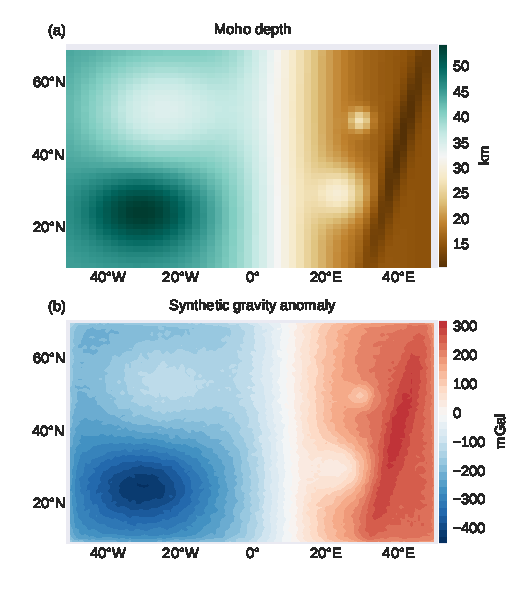
\includegraphics{figures/synthetic-simple-data}
    \caption{
        A simple Moho model made of tesseroids for synthetic data application.
        (a) The Moho depth of the model in kilometers.
        The model transitions from a deep Moho in the right to a shallow Moho in
        left, simulating the transition between a continental and an oceanic
        Moho.
        Each pixel in the pseudo-color image corresponds to a tesseroid of the
        model.
        (b) Noise-corrupted synthetic gravity data generated from the model
        shown in (a).
    }
    \label{fig:simple-data}
\end{figure}

\begin{figure*}
    \centering
    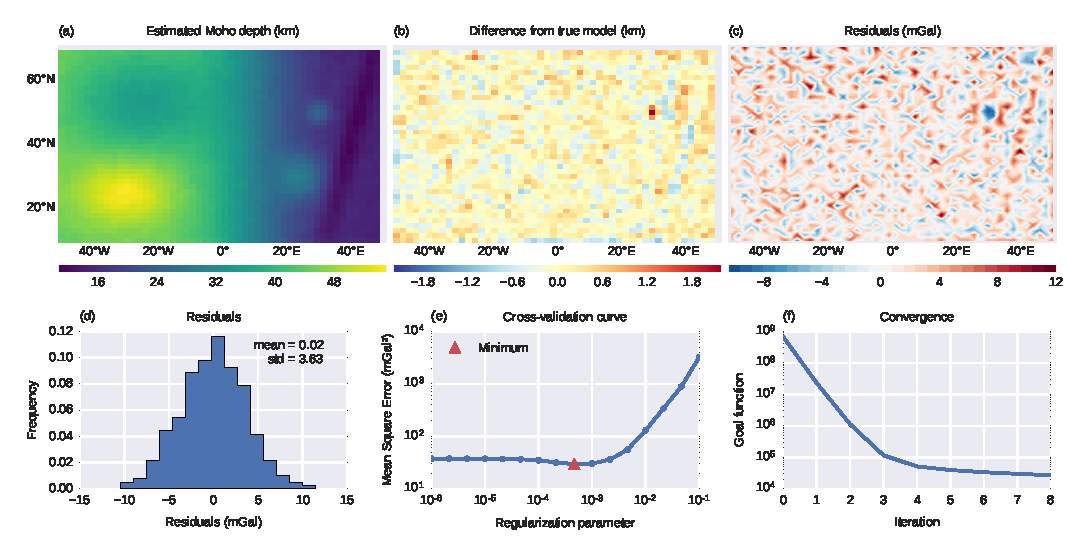
\includegraphics[width=\textwidth]{figures/synthetic-simple-results}
    \caption{
        Results from the inversion of the simple synthetic data.
        (a) The estimated Moho depth.
        (b) The difference between the true model depths
        and the estimated depths.
        (c) The inversion residuals (observed data minus
        the data predicted by the estimate).
        (d) Histogram of the residuals. Also shown are the calculated
        mean and standard deviation (std) of the residuals.
        Note that the data were contaminated with normally distributed
        pseudo-random noise with zero mean and 5 mGal standard deviation.
        (e) Cross-validation curve used to determine the optimal regularization
        parameter (Eq.~\ref{eq:goalfunction}).
        Both axis are in logarithmic scale.
        The minimum Mean Square Error (Eq.~\ref{eq:msemu}) is found at
        $\mu = 0.00046$ (red triangle).
        (f) Goal function value (Eq.~\ref{eq:goalfunction}) per Gauss-Newton
        iteration showing the convergence of the gradient descent.
        The y-axis is in logarithmic scale.
    }
    \label{fig:simple-results}
\end{figure*}

We simulate the transition from a continental-type Moho to an oceanic-type Moho
using a model composed of $M_{lat} \times M_{lon} = 40 \times 50$ grid of
juxtaposed tesseroids (a total of $M = 2000$ model elements).
The anomalous Moho density-contrast is $\Delta\rho = 400\ kg/m^3$
and the Normal Earth Moho depth is $z_{ref} = 30\ km$.
Fig.~\ref{fig:simple-data}a shows the model Moho depths,
where each pixel in the pseudo-color image corresponds to
a tesseroid of the model.

The synthetic data were forward modeled on a regular grid of
$N_{lat} \times N_{lon} = 79 \times 99$ points
(a total of $N = 7821$ observations)
at a constant height of 50 km.
The data were contaminated with pseudo-random noise
sampled from a normal distribution with zero mean and 5 mGal standard deviation.
Fig.~\ref{fig:simple-data}b shows the noise-corrupted full synthetic data set.
The data grid spacing is half the grid spacing of the tesseroid model
so that, when separating the training and testing data sets
(Fig.~\ref{fig:grid_separation}),
the training data set points will fall directly above each model element.

We separated the synthetic data into training and testing data sets
following Fig.~\ref{fig:grid_separation}.
The training data set is a regular grid of
$N_{lat} \times N_{lon} = 40 \times 50$ points
(a total of $N_{train} = 2000$).
The testing data set is composed of $N_{test} = 5821$ observations.
We used cross-validation to estimate an optimal regularization parameter ($\mu$)
from a set of $N_\mu = 16$ values equally spaced on a logarithmic scale
between $10^{-6}$ and $10^{-1}$.
We ran our regularized inversion on the training data set
for each value of $\mu$,
obtaining 16 Moho depth estimates.
For all inversions, the initial Moho depth estimate
used to start the Gauss-Newton optimization
was set to 60 km depth for all inversion parameters.
Furthermore, $z_{ref}$ and $\Delta\rho$ are set to their respective true values.
Finally, we computed the mean square error (MSE, Eq.~\ref{eq:msemu})
for each estimate and chose as the final estimated Moho model
the one that minimizes the MSE.

Fig.~\ref{fig:simple-results} summarizes the inversion results.
Fig.~\ref{fig:simple-results}a shows the final estimated Moho depth
after cross-validation.
The recovered model is smooth, indicating that the cross-validation procedure
was effective in estimating an optimal regularization parameter.
Fig.~\ref{fig:simple-results}b shows difference between the true Moho depth
(Fig.~\ref{fig:simple-data}a) and the estimated Moho depth.
The differences appear to be semi-randomly distributed with a maximum
coinciding with a short-wavelength feature in the true model.
The maximum and minimum differences are approximately
2.19 and -2.13 km, respectively.
Fig.~\ref{fig:simple-results}c shows inversion residuals (difference between
the observed and predicted data), in mGal.
The largest residual (in absolute value) coincides with the largest difference
between the true model and the estimate.
The inversion residuals are normally distributed,
as shown in Fig.~\ref{fig:simple-results}d,
with 0.02 mGal mean and a standard deviation of 3.63 mGal.
The cross-validation curve in Fig.~\ref{fig:simple-results}e
shows a clear minimum MSE at $\mu = 0.00046$
(indicated by the red triangle).
Fig.~\ref{fig:simple-results}f shows the convergence of
the Gauss-Newton optimization in eight iterations.

We also investigated the computation time spent in each section of the inversion
process using a source code profiler.
The profiler measures how much time is spent inside each function during
the execution of a program.
We ran the profiler on a single inversion of the training data set
using the estimated regularization parameter.
We tracked the total time spent inside each of the three functions
that represent the largest computational bottlenecks of the inversion:
solving the linear system in Eq.~\ref{eq:gaussnewton-regul}
using the conjugate gradient method,
performing the dot products required to compute
the Hessian matrix (Eq.~\ref{eq:hessian-regul})
and the gradient vector (Eq.~\ref{eq:gradient-regul}),
and forward modeling to calculate the predicted data (Eq.~\ref{eq:forward}).
The profiling results presented in Table~\ref{profiling}
show that the time spent on forward modeling accounts for approximately
99.8\% of the total computation time.


% Insert the profiling results table

\begin{table}
    \centering
    \caption{
        Time spent on each function during a single inversion of
        simple synthetic data.
        The inversion was performed on a laptop computer with a
        Intel(R) Core(TM) i7-3612QM CPU @ 2.10GHz processor.
        The total time for the inversion was 42.133 seconds.
    }
    \label{profiling}
    \begin{tabular}{lcc}
        Function description & Time (s) & Percentage of total time (\%)\\
        \hline
        Sparse conjugate gradient & 0.021 & 0.050\\
        Sparse dot product & 0.007 & 0.017\\
        Tesseroid forward modeling & 42.059 & 99.824\\
        \hline
    \end{tabular}
\end{table}





%%%%%%%%%%%%%%%%%%%%%%%%%%%%%%%%%%%%%%%%%%%%%%%%%%%%%%%%%%%%%%%%%%%%%%%%%%%%%%%
\subsection{Model based on CRUST1.0}\label{sec:crust1}

\begin{figure*}
    \centering
    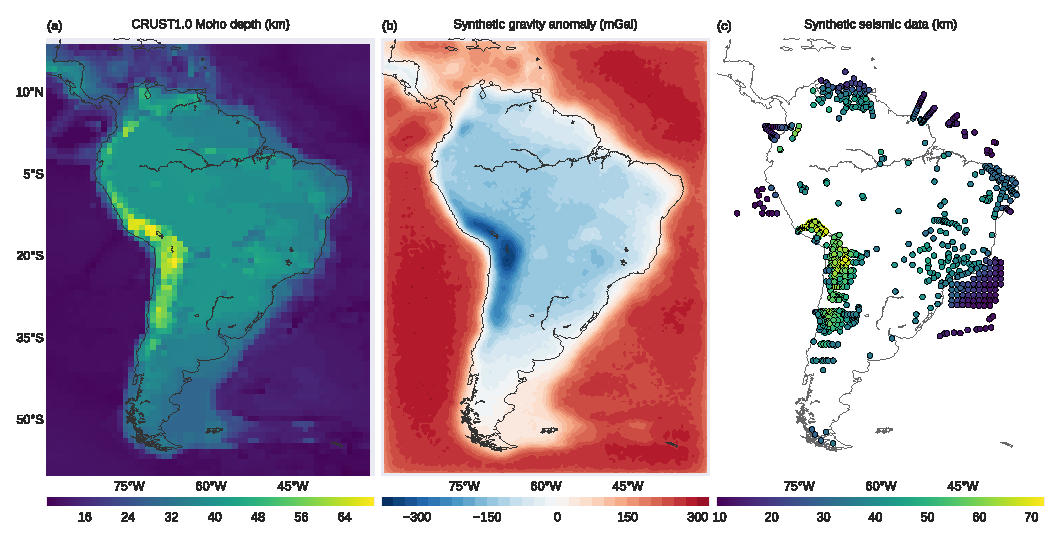
\includegraphics[width=\textwidth]{figures/synthetic-crust1-data}
    \caption{
        Synthetic data of a model derived from CRUST1.0.
        The model is made of tesseroids with an constant density-contrast
        of $\Delta\rho = 350\ kg/m^3$ and assuming a reference level of
        $z_{ref} = 30\ km$.
        (a) The Moho depth of the model in kilometers.
        Each pixel in the pseudo-color image corresponds to a tesseroid of the
        model.
        (b) Noise-corrupted synthetic gravity data generated from the model.
        (c) Synthetic seismic data simulating point estimates of Moho depth.
        The point estimates were obtained by interpolating
        the Moho depth in (a).
    }
    \label{fig:crust1-data}
\end{figure*}

\begin{figure*}
    \centering
    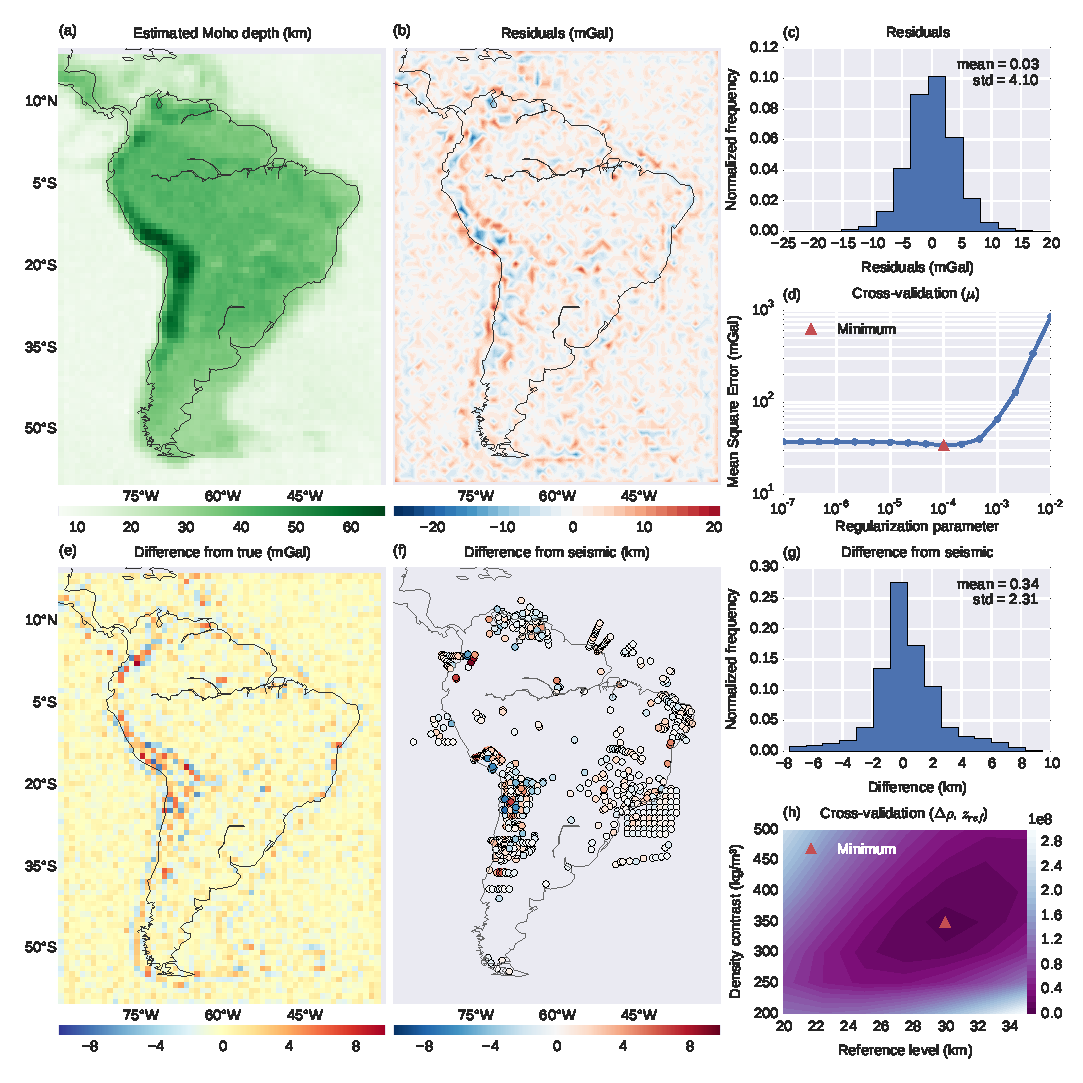
\includegraphics[width=\textwidth]{figures/synthetic-crust1-results}
    \caption{
        Inversion results from the CRUST1.0 synthetic data.
        (a) Cross-validation curve used to determine
        the regularization parameter (Eq.~\ref{eq:goalfunction}).
        The minimum Mean Square Error (Eq.~\ref{eq:msemu}) is found at
        $\mu = 0.0001$ (red triangle).
        (b) Cross-validation results used to determine
        the reference level ($z_{ref}$) and the density-contrast ($\Delta\rho$).
        The colored contours represent
        the Mean Square Error (Eq.~\ref{eq:msehyper}) in $km^2$.
        The minimum (red triangle) is found at $z_{ref} = 30\ km$
        and $\Delta\rho = 350\ kg/m^3$.
        (c) The estimated Moho depth.
        (d) Difference between the CRUST1.0 model depths
        (Fig.~\ref{fig:crust1-data}a)
        and the estimated depths.
        (e) Histogram of the inversion residuals
        (observed minus predicted data).
        (f) Histogram of the differences between
        the synthetic seismic observations (Fig.~\ref{fig:crust1-data}c)
        and the estimated depths.
        (g) The inversion residuals.
        (h) Difference between the seismic and the estimated depths.
    }
    \label{fig:crust1-results}
\end{figure*}


In this test, we simulate the anomalous Moho of South America
using Moho depth information extracted from the CRUST1.0 model
\citep{laske2013}.
We construct a tesseroid model with
$M_{lat} \times M_{lon} = 80 \times 60$ juxtaposed elements, 4800 in total,
using the Moho depths shown in Fig.~\ref{fig:crust1-data}a.
In our model, the Normal Earth Moho is $z_{ref} = 30\ km$ and
the density-contrast is $\Delta\rho = 350\ kg/m^3$.
We produce the synthetic data at a constant height of 50 km
and on a regular grid of $N_{lat} \times N_{lon} = 159 \times 119$ points
(a total of 18921 observations).
We contaminate the synthetic data with normally distributed pseudo-random noise
with zero mean and 5 mGal standard deviation (Fig.~\ref{fig:crust1-data}b).

The cross-validation procedure to determine $\Delta\rho$ and $z_{ref}$
requires knowledge of the Moho depth at certain points
($\mathbf{z}_s^o$ in Eq.~\ref{eq:msehyper}),
usually from seismic experiments.
Thus, we must also generate synthetic seismic data about the Moho depth.
We produce such data by interpolating the Moho depth shown in
Fig.~\ref{fig:crust1-data}a on the same geographic coordinates
as the 937 points from the \citet{assumpcao2013a} data set.
The resulting synthetic seismic data is shown in Fig.~\ref{fig:crust1-data}c.

We perform the cross-validation procedures in two parts.
First, we run the cross-validation to estimate
an optimal regularization parameter ($\mu$).
The starting estimate for all inversions is
60 km depth for all model parameters.
For this cross-validation,
we keep $z_{ref}$ and $\Delta\rho$ fixed to
$20\ km$ and $500\ kg/m^3$, respectively.
Our investigations suggest that the outcome of this round of cross-validation
does not depend on the particular values of $z_{ref}$ and $\Delta\rho$ used.
Second, we use the estimated $\mu$ to run the cross-validation
to estimate $z_{ref}$ and $\Delta\rho$,
thus obtaining the final estimated Moho depths.
Fig.~\ref{fig:crust1-results} summarizes the results
from both cross-validation runs and the final inversion results.

For the first cross-validation,
we separate the synthetic data (Fig.~\ref{fig:grid_separation}) into
a training set with twice the grid spacing of the original data
($N_{lat} \times N_{lon} = 80 \times 60$)
and a testing set with 14,121 observations.
We run the inversion for 16 different values of $\mu$
equally spaced in a logarithmic scale between $10^{-7}$ and $10^{-2}$.
For each of the 16 estimates we compute the MSE (Eq.~\ref{eq:msemu}),
shown in Fig.~\ref{fig:crust1-results}a as function of $\mu$.
The optimal regularization parameter that minimizes the MSE is $\mu = 10^{-4}$
(indicated by the red triangle).

In the second cross-validation,
we use the estimated value of $\mu$ in all inversions.
We test seven values of $z_{ref}$ from 20 to 35 km with 2.5 km intervals
and seven values of $\Delta\rho$ from 200 to 500 $kg/m^3$
with 50 $kg/m^3$ intervals.
We run the inversion for every combination of $z_{ref}$ and $\Delta\rho$,
totaling 49 inversions.
Finally, we calculate the Mean Square Error (Eq.~\ref{eq:msehyper})
for each of the 49 estimates
and choose the values of $z_{ref}$ and $\Delta\rho$ that minimize the MSE.
Fig.~\ref{fig:crust1-results}b
shows a colored-contour map of the MSE
with a minimum (marked by the red triangle)
at $z_{ref} = 30\ km$ and $\Delta\rho = 350\ kg/m^3$.

Fig.~\ref{fig:crust1-results}c shows the final solution after both
cross-validation procedures.
The recovered model is smooth, indicating that the cross-validation procedure
was effective in estimating an optimal regularization parameter.
Fig.~\ref{fig:crust1-results}d shows the difference between
the true Moho depths (Fig.~\ref{fig:crust1-data}a)
and the estimated depths.
The maximum and minimum differences are, respectively,
9.8 and -8.2 km.
The largest absolute differences are located along the central and northern
Andes, where there is a sharp increase in the true Moho depth
(Fig.~\ref{fig:crust1-data}a).
Positive differences (indicating a too shallow estimate)
appear along the central portion of the Andes,
flanked by regions of negative differences (indicating a too deep estimate)
on the continental and Pacific sides.
Figs.~\ref{fig:crust1-results}e and g show the inversion residuals (difference
between the observed and predicted data).
The inversion residuals appear normally distributed,
with 0.03 mGal mean and a standard deviation of 4.10 mGal.
The residuals follow a similar, though reversed, pattern
to the differences shown in Fig.~\ref{fig:crust1-results}d.
The largest residuals (in absolute value) are along the Andes,
with the central portion being dominated by negative residuals
and flanked by positive residuals on both sides.
Figs.~\ref{fig:crust1-results}f and h show the differences between
the synthetic seismic data (Fig.~\ref{fig:crust1-data}c)
and the estimated Moho depths.
Once more, the largest differences are concentrated along the Andes,
particularly in the central Andes and near Ecuador and Colombia.
The differences are smaller along the Atlantic coast of South America,
with notable larger differences in a few points of northeastern Brazil
and along the Amazon river.
In general, large residuals are associated with sharp increases in Moho depth.



%%%%%%%%%%%%%%%%%%%%%%%%%%%%%%%%%%%%%%%%%%%%%%%%%%%%%%%%%%%%%%%%%%%%%%%%%%%%%%%
\section{Application to the South American Moho}


We apply the inversion method proposed here to invert for the Moho depth of the
South American continent.
We follow the application of \citet{vandermeijde2013} but with some
differences, mainly using a different data set and performing all modeling
in spherical coordinates using tesseroids.
The data are corrected of the effects of topography and sedimentary basins.
Crust and mantle heterogeneities cannot be properly accounted for
in regions where information coverage is sparse and readily accessible models
are not available, like in South America and Africa.
Hence, for the purposes of this study, we will assume to be negligible all
other crustal and mantle sources, including lateral variations in density along
the Moho.


%%%%%%%%%%%%%%%%%%%%%%%%%%%%%%%%%%%%%%%%%%%%%%%%%%%%%%%%%%%%%%%%%%%%%%%%%%%%%%%
\subsection{Gravity and seismic data}

\begin{figure*}
    \centering
    \includegraphics[width=\textwidth]{figures/south-america-corrections}
    \caption{
        Gravity data for South America and the models used in the data
        corrections.
        (a) The gravity disturbance (Eq.~\ref{eq:disturbance}) calculated from
        the raw gravity data.
        (b) Topography from ETOPO1.
        (c) Gravitational attraction of the topography calculated
        at the observation height using tesseroids.
        (d) The Bouguer disturbance (Eq.~\ref{eq:bouguer}) obtained by
        subtracting (c) from (a).
        The upper (e), middle (f), and lower (g) sediment layer thicknesses
        from the CRUST1.0 model.
        (h) The total gravitational attraction of the sediment layers shown in
        (e), (f), and (g), calculated using tesseroids.
        }
    \label{fig:sam-corrections}
\end{figure*}

\begin{figure*}
    \centering
    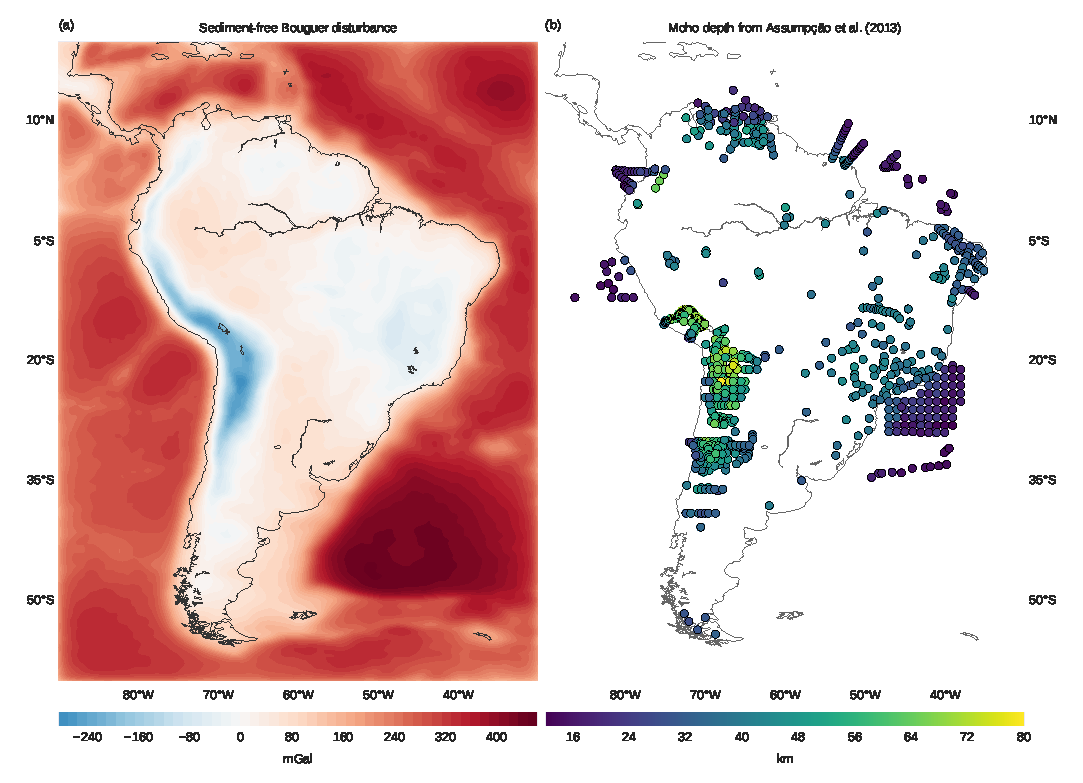
\includegraphics[width=\textwidth]{figures/south-america-data}
    \caption{
        Input data for the South American Moho inversion.
        (a) Sediment-free Bouguer disturbance for South America.
        Obtained by subtracting the total sediment gravitational effect
        (Fig.~\ref{fig:sam-corrections}h) from the Bouguer disturbance
        (Fig.~\ref{fig:sam-corrections}d).
        (b) Seismological Moho depth estimates from
        \citet{assumpcao2013a}.
    }
    \label{fig:sam-data}
\end{figure*}


The raw gravity data are generated from the satellite only
spherical harmonic model GOCO5S \citet{mayer-guerr2015}.
The GOCO5S model combines data from 15 satellites, including the complete
mission data from the GOCE satellite.
The data were downloaded from the
International Centre for Global Earth Models (ICGEM) web-service
\citep[][ \url{http://icgem.gfz-potsdam.de/ICGEM/})]{barthelmes2012}
in the form of the complete gravity field
on a regular grid with $0.2^\circ$ grid spacing at ellipsoidal height 50 km.
We calculate the gravity disturbance
($\delta(P)$ in Eq.~\ref{eq:disturbance})
by subtracting from the raw data
the normal gravity of the WGS84 reference ellipsoid ($\gamma(P)$)
using the formula of \citet{li2001a}.
Fig.~\ref{fig:sam-corrections}a show the calculated gravity disturbance of
South America.

We remove the gravitational effect of the topography
from the gravity disturbance
by modeling the ETOPO1 digital terrain model
\citep[][ \url{http://dx.doi.org/10.7289/V5C8276M}]{amante2009}
using tesseroids (Fig.~\ref{fig:sam-corrections}b).
We used the standard densities of $2670\ kg/m^3$ for continents and
$-1630\ kg/m^3$ for the oceans.
Fig.~\ref{fig:sam-corrections}c shows the calculated gravitational attraction
of the topographic masses at 50 km height.
Fig.~\ref{fig:sam-corrections}d shows the Bouguer disturbance
(Eq.~\ref{eq:bouguer}) obtained after subtracting the topographic effect from
the gravity disturbance.

The effect of sedimentary basins is removed using
tesseroid models of the three sedimentary layers present in the CRUST1.0 model
\citep[][ \url{http://igppweb.ucsd.edu/~gabi/rem.html}]{laske2013}.
Each sedimentary layer model includes the density
of each $1^\circ \times 1^\circ$ model cell.
Figs.~\ref{fig:sam-corrections}e-g show the thickness of the upper, middle, and
lower sedimentary layers, respectively.
The density-contrasts of the tesseroid model is obtained by subtracting
$2670\ kg/m^3$ from the density of each model element.
Fig.~\ref{fig:sam-corrections}h shows the combined gravitational attraction of
the sedimentary basin tesseroid model.
We subtract the total effect of sediments from the Bouguer disturbance in
Fig.~\ref{fig:sam-corrections}d to obtain
the sediment-free Bouguer disturbance (Fig.~\ref{fig:sam-data}a),
which will be used as input for the inversion.

The seismic point estimates of Moho depth used in the cross-validation
procedure are from the data set of \citet{assumpcao2013a}.
The 937 data points in this data set are shown in Fig.~\ref{fig:sam-data}b.


%%%%%%%%%%%%%%%%%%%%%%%%%%%%%%%%%%%%%%%%%%%%%%%%%%%%%%%%%%%%%%%%%%%%%%%%%%%%%%%
\subsection{Inversion and cross-validation}

\begin{figure}
    \centering
    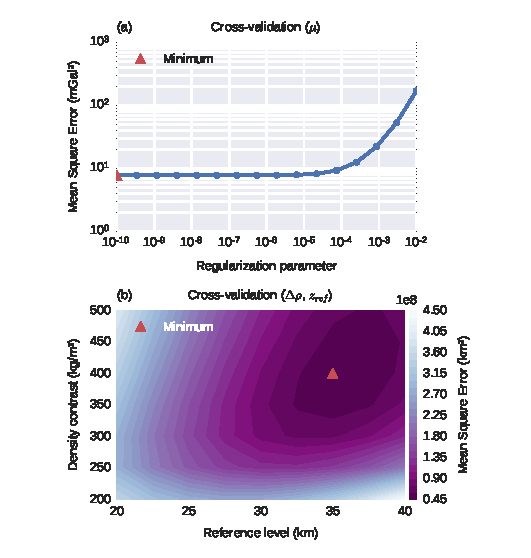
\includegraphics{figures/south-america-cv}
    \caption{
        Cross-validation results for the South American Moho inversion.
        (a) Cross-validation to determine the regularization parameter $\mu$
        (Eq.~\ref{eq:goalfunction}).
        The minimum Mean Square Error (Eq.~\ref{eq:msemu}),
        shown as a red triangle,
        corresponds to $\mu = 10^{-10}$.
        (b) Cross-validation to determine
        the reference level ($z_{ref}$) and the density-contrast ($\Delta\rho$).
        The colored contours represent
        the Mean Square Error (Eq.~\ref{eq:msehyper}).
        The minimum (red triangle) is found at $z_{ref} = 35\ km$
        and $\Delta\rho = 400\ kg/m^3$.
    }
    \label{fig:sam-cv}
\end{figure}



As in the CRUST1.0 synthetic data test (section~\ref{sec:crust1}),
we perform the cross-validation in two parts.
First, we run the cross-validation to estimate
an optimal regularization parameter ($\mu$).
The starting estimate for all inversions is
60 km depth for all model parameters.
For this cross-validation,
we keep $z_{ref}$ and $\Delta\rho$ fixed to
$20\ km$ and $500\ kg/m^3$, respectively.
Second, we use the estimated $\mu$ to run the cross-validation
to estimate $z_{ref}$ and $\Delta\rho$,
thus obtaining the final estimated Moho depth model.

We split the sediment-free gravity data into the training and testing data
sets.
The training data set is a regular grid with $0.4^\circ$ grid spacing
(twice the spacing of the original data grid)
and $N_{lat} \times N_{lon} = 201 \times 151$ grid points,
a total of 30,351 observations.
The remaining 90,350 points compose the testing data set.
We test 16 values of the regularization parameter ($\mu$)
equally spaced on a logarithmic scale between $10^{-10}$ and $10^{-2}$.
Fig.~\ref{fig:sam-cv}a shows the Mean Square Error (MSE)
as a function of $\mu$.
The minimum MSE is found at $\mu = 10^{-10}$, the lowest value of $\mu$ tested,
suggesting that little or no regularization is required.

We proceed with the second cross-validation using $\mu = 10^{-10}$ in all
inversions.
We test all combinations of
seven values of $z_{ref}$, from 20 to 35 km with 2.5 km intervals,
and seven values of $\Delta\rho$, from 200 to 500 $kg/m^3$
with 50 $kg/m^3$ intervals.
Fig.~\ref{fig:sam-cv}b shows a map of the MSE
with respect to the \citet{assumpcao2013a} data set.
The MSE has a well defined minimum, indicated by the red triangle,
at $z_{ref} = 35\ km$ and $\Delta\rho = 400\ kg/m^3$.


%%%%%%%%%%%%%%%%%%%%%%%%%%%%%%%%%%%%%%%%%%%%%%%%%%%%%%%%%%%%%%%%%%%%%%%%%%%%%%%
\subsection{Moho model for South America}

\begin{figure*}
    \centering
    
\includegraphics[width=\textwidth]{figures/south-america-moho}
    \caption{
        Inversion results for the South American Moho.
        (a) The estimated Moho depth of South America.
        The solid light grey line is the 35 km Moho depth contour.
        (b) Inversion residuals (observed data in Fig.~\ref{fig:sam-data}a
        minus the data predicted by the estimate (a)).
        (c) Differences between the seismological depths of
        \citet{assumpcao2013a} and our gravity-derived estimate shown in (a).
        The inset in (c) shows a histogram of the differences along with their
        calculated mean and standard deviation (std).
    }
    \label{fig:sam-moho}
\end{figure*}


The final Moho depth model for South America is shown
as a pseudo-color map in Fig.~\ref{fig:sam-moho}a.
The model is available in the online repository that accompanies
this contribution (see section~\ref{sec:software}).
Each model element is a $0.4^\circ \times 0.4^\circ$ tesseroid,
represented by the pixels in the pseudo-color map.

Our model differs significantly from CRUST1.0 (Fig.~\ref{fig:crust1-data}a)
but contains most of the large-scale features
present in the GMSA12 gravity-derived model of \citet{vandermeijde2013}.
The deepest Moho is along the central Andes, reaching depths upward of 70 km.
The oceanic areas present the shallowest Moho, ranging approximately
from 7.5 to 20 km.
The Brazilian and Guiana shields have a deeper Moho (greater than 35 km),
with the deepest portion in the area of the São Francisco craton.
The Moho is shallower than 35 km along the western Amazon and Andean foreland
regions, as well as along the Amazon river.

Fig.~\ref{fig:sam-moho}b shows the inversion residuals
(observed minus predicted data)
and Fig.~\ref{fig:sam-moho}c shows the differences between
the seismic-derived depths of \citet{assumpcao2013a}
(Fig.~\ref{fig:sam-data}b) and the depths in our model.
The differences range from approximately -23 to 23 km
and have a mean of 1.18 km and a standard deviation of 6.84 km.
The residuals and differences from seismic are smallest in the oceanic areas,
southern Patagonia, and the eastern coast of the continent.
The largest residuals are located along the Andes and correlate with the
deepest Moho depths.
These large residuals follow a pattern of a negative value in the center
flanked by positive values to the East and West.
This same pattern is observed in the CRUST1.0 synthetic test results
(Fig.~\ref{fig:crust1-results}),
suggesting that this is a byproduct of the inversion method, not the data.
Likewise, larger residuals also appear to be associated with sharp variations
in the estimated Moho depth.
Along the Andes, large differences with seismic data are correlated with the
large inversion residuals.
Conversely, this correlation is absent from the large differences seen in
points around Venezuela.
In the Borborema province, northeastern Brazil,
our model slightly overestimates the Moho depth.
On the other hand, our model underestimates the depths
in the Amazon region and the Paraná Basin.
Particularly in the Amazon Basin,
where our model predicts a Moho depth of approximately 30 km,
the residuals and the differences with the seismic data are larger than in the
Paraná Basin.



%%%%%%%%%%%%%%%%%%%%%%%%%%%%%%%%%%%%%%%%%%%%%%%%%%%%%%%%%%%%%%%%%%%%%%%%%%%%%%%
\section{Conclusions}

We have developed a computationally efficient gravity inversion method in
spherical coordinates.
Our method extends the Gauss-Newton formulation of Bott's method
\citep{silva2014} to use tesseroids as model elements and smoothness
regularization.
We retain the computational efficiency of Bott's method by taking advantage of
the sparse nature of all matrices involved.
We employ two cross-validation techniques to estimate the hyper-parameters of
the inversion: the regularization parameter, the Moho density-contrast, and the
Normal Earth Moho depth.

The test on simple synthetic data shows that our inversion method is able to
recover a smooth Moho relief with a homogeneous density-contrast.
The inversion was not able to fully recover the shortest wavelength feature in
the model, possibly due to the smoothness constraints which tends to soften
high-frequency (sharp) variations.
The cross-validation Mean Square Error curve in Fig.~\ref{fig:simple-results}e
has a well-defined minimum, indicating a value of the regularization parameter
($\mu$) whose corresponding estimate best predicts data that were not included
in the inversion.
Using this value of $\mu$ in the inversion leads to a smooth Moho relief and
acceptable data misfit.

The source code profiling results presented in Table~\ref{profiling}
confirm the efficiency of the proposed method.
When using sparse matrices, solving linear systems and performing matrix
multiplications together account for a mere 0.067\% of the total computation
time required for a single inversion.
The majority of the computation time (99.824\%) is spent on forward modeling.
Thus, we are able to retain the high computational efficiency of Bott's method
while using a classic Tikhonov regularization formulation.
This approach could, in theory, be extended to other types of regularization
(e.g., Total Variation) and misfit functions (e.g., re-weighted least squares)
already available in the literature.
For example, the Total Variation approach used by \citet{martins2011} could
potentially be implemented in a more straight forward manner than done by
\citet{santos2015}.

The more complex synthetic data test based on CRUST1.0
(Fig.~\ref{fig:crust1-results})
shows that the cross-validation using pointwise Moho depth information
is able to correctly estimate the density-contrast ($\Delta\rho$) and Normal
Earth Moho depth ($z_{ref}$).
This test indicates that the inversion neither correctly estimates Moho depth
nor adequately fits the gravity and pointwise data when sharp variations in
Moho depth occur.
This phenomenon is particularly strong in the region below the Andes.
A likely explanation is that the smoothness regularization
is intrinsically unable to produce sharp variations in Moho depth.
These effects might be mitigated with the use of sharpness-inducing
regularization, like Total Variation \citep{martins2011},
Cauchy norm regularization \citep{sacchi1996, pilkington2008},
or an adaptive mixed smoothness-sharpness regularization \citep{sun2014}.

We applied the method proposed here to estimate the Moho depth for South
America.
Our Moho depth model is in accordance with previous results by
\citet{vandermeijde2013}.
The model fits well the gravity and seismic data in all oceanic regions, the
central portion of the Andean foreland, Patagonia, and coastal and central
parts of Brazil.
However, the model is unable to fit the gravity and seismic data in places with
sharp variations in Moho depth, particularly below the Andes.
This might indicate the improper use of smoothness regularization, as suggested
by the CRUST1.0 synthetic data test, or the presence of crustal or mantle
density anomalies that were unaccounted for during the data corrections.
In the coastal region of Venezuela, along the central Amazon and Solimões
Basins, and in the Paraná Basin, the model is able to fit the gravity data but
differs significantly from the seismic data.
\citet{mariani2013} and \citet{nunn1988} explain these discrepancies in the
Paraná and Amazon Basins, respectively, as high density rocks in the lower
crust.
In general, differences between a gravity and a seismically derived Moho model
may indicate the presence of crustal or mantle density anomalies that were
unaccounted for in the data processing.
Such locations warrant further detailed investigation.



%%%%%%%%%%%%%%%%%%%%%%%%%%%%%%%%%%%%%%%%%%%%%%%%%%%%%%%%%%%%%%%%%%%%%%%%%%%%%%%
\section{Acknowledgments}

We are indebted to the developers and maintainers of the open-source
software without which this work would not have been possible.
L. Uieda was supported by a scholarship from
Coordenação de Aperfeiçoamento de Pessoal de Nível Superior
(CAPES).
V.C.F. Barbosa was supported by a fellowship from
Conselho Nacional de Desenvolvimento Científico e Tecnológico (CNPq).
\todo{Coloco o projeto da FAPERJ também?}

%%%%%%%%%%%%%%%%%%%%%%%%%%%%%%%%%%%%%%%%%%%%%%%%%%%%%%%%%%%%%%%%%%%%%%%%%%%%%%%

\bibliographystyle{gji}
\bibliography{biblio}

\end{document}
